\subsection{Question 1}
\subsubsection{Part A}

Method 1: \(LU\) factor \(A-sI\) for \(s=0\) and \(s=1\) and inspecting the number of negative values on the diagonal of \(U\).

Case 1: \(s=0\),

\begin{eqnarray}
  A_0 = 
  \begin{pmatrix}
    -1 & 1 & 0 \\
    1 & 1 & 1 \\
    0 & 1 & 2 \\
  \end{pmatrix}
\end{eqnarray}

\begin{eqnarray}
  L_0 =
  \begin{bmatrix}
    1 & 0 & 0 \\
    -1 & 1 & 0 \\
    0 & 0 & 1 \\
  \end{bmatrix}
  , U_0 =
  \begin{bmatrix}
    -1 & 1 & 0 \\
    0 & 2 & 1 \\
    0 & 0 & 1.5 \\
  \end{bmatrix}
  \\
  L_1 = 
  \begin{bmatrix}
    1 & 0 & 0 \\
    -1 & 1 & 0 \\
    0 & 0.5 & 1 \\
  \end{bmatrix}
  , U_1 = 
  \begin{bmatrix}
    -1 & 1 & 0 \\
    0 & 2 & 1 \\
    0 & 0 & 1.5 \\
  \end{bmatrix}
\end{eqnarray}

Therefore, when we inpsect the diagonal of \(U_1\) we see that there is one negative value.
This means that there is one eigenvalue in \(A\) that is less than zero.

Case 2: \(s=1\),


\begin{eqnarray}
  A_1 = 
  \begin{pmatrix}
    -2 & 1 & 0 \\
    1 & 0 & 1 \\
    0 & 1 & 1 \\
  \end{pmatrix}
\end{eqnarray}

\begin{eqnarray}
  L_0 =
  \begin{bmatrix}
    1 & 0 & 0 \\
    -0.5 & 1 & 0 \\
    0 & 0 & 1 \\
  \end{bmatrix}
  , U_0 =
  \begin{bmatrix}
    -2 & 1 & 0 \\
    0 & 0.5 & 1 \\
    0 & 1 & 1 \\
  \end{bmatrix}
  \\
  L_1 = 
  \begin{bmatrix}
    1 & 0 & 0 \\
    -0.5 & 1 & 0 \\
    0 & 2 & 1 \\
  \end{bmatrix}
  , U_1 = 
  \begin{bmatrix}
    -2 & 1 & 0 \\
    0 & 0.5 & 1 \\
    0 & 0 & -1 \\
  \end{bmatrix}
\end{eqnarray}

Therefore, when we inpsect the diagonal of \(U_1\) we see that there are two negative values.
This means that there are two eigenvalues in \(A\) that are less than one.
Utilizing the knowledge from both cases we have found that there is one eigenvalue in the range \([0,1]\).
\newpage
Method 2: Compute the number of sign changes in the sequence of main principal minors of \(A-sI\) for \(s=0\) and \(s=1\).

\lstinputlisting[caption=Matlab Commands,showstringspaces=false,language=Matlab]{../mpm.m}
\lstinputlisting[caption=Matlab Commands,showstringspaces=false,language=Matlab]{../q1_partA}

We see that in case 1 there is one sign change in the sequence of main principal minors and that in case 2 there are two sign changes in the sequence of main principal minors.
Therefore, as with method 1 we have shown there is a single eigenvalue in the range \([0,1]\).

\subsubsection{Part B}

The best estimate count of arthmetic operations for the two methods was 116 flops for method 1 and 36 flops for method 2.
Therefore, it would seem that method 2 is more efficient for tri-diagonal matrices and it makes intuitive sense that this gap will become larger as the matrices grow in size ({\em i.e.,} method 2 will look better and better relative to method 1).

\newpage
\subsubsection{Part C}

The code below generates 100 symmetric tridiagonal matrices of size 50x50 and runs both Method 1 and Method 2 from part A.
\lstinputlisting[caption=Matlab Commands,showstringspaces=false,language=Matlab]{../q1_partC.m}

The results of the code snippet above are presented below.
It is clear as stated in part B that Method 2 dominates Method 1 in terms of running speed.
This contrast grows as the size of the symmetric tridiagonal matrix grows.
\lstinputlisting[caption=Matlab Commands,showstringspaces=false,language=Matlab]{../q1_partC}

\newpage
\subsection{Question 2}
\subsubsection{Part A}

Since the Gerschgorin's disks are pairwise disjoint we know that each disk must contain one eigenvalue.
Therefore the cardinality of \(\sigma(A) = n\).
This means that the algebraic multiplicity \(m_a\) of each eigenvalue is \(m_a = 1\).
We know that the geometric multiplicity \(m_g\) follows the rule \(m_g \leq m_a\) for all eigenvalues of \(A\).
Therefore, since \(m_a = 1\) we can say that \(m_g = 1\). 

\subsubsection{Part B}

Leon is correct because as stated above \(m_g = m_a\) for eigenvalues of \(A\).


\subsubsection{Part C}

Nina is correct because there are \(n\) eigenvalues; one per disk.
If there was a complex eigenvalue it's complex conjugate would be an eigenvalue as well.
This would require two eigenvalues to be loacted in a single disk.
However this would contradict what we have shown in (a).
Therefore all eigenvalues of \(A\) are real.

\subsubsection{Part D}

Elvis is not correct.
The problem is that there can be two distinct eigenvalues in the real that have the same magnitude.
For example, suppose a matrix \(B\) as eigenvalues \(\lambda_{1} = 6, \lambda_{2} = -6\).
It is clear, \(|\lambda_{1}| = |\lambda_{2}|\).
In this case the power method will not converge because there is no dominant eigenvalue.

\newpage
\subsection{Question 3}

\lstinputlisting[caption=Matlab Commands,showstringspaces=false,language=Matlab]{../q3.m}
\lstinputlisting[caption=Matlab Commands,showstringspaces=false,language=Matlab]{../q3_results}

\newpage
\subsection{Question 4}
\subsubsection{Part A}
\subsubsection{Part B}

%\lstinputlisting[caption=Matlab Commands,showstringspaces=false,language=Matlab]{../lu_sym.m}

%\begin{figure}[th]
%  \centering
%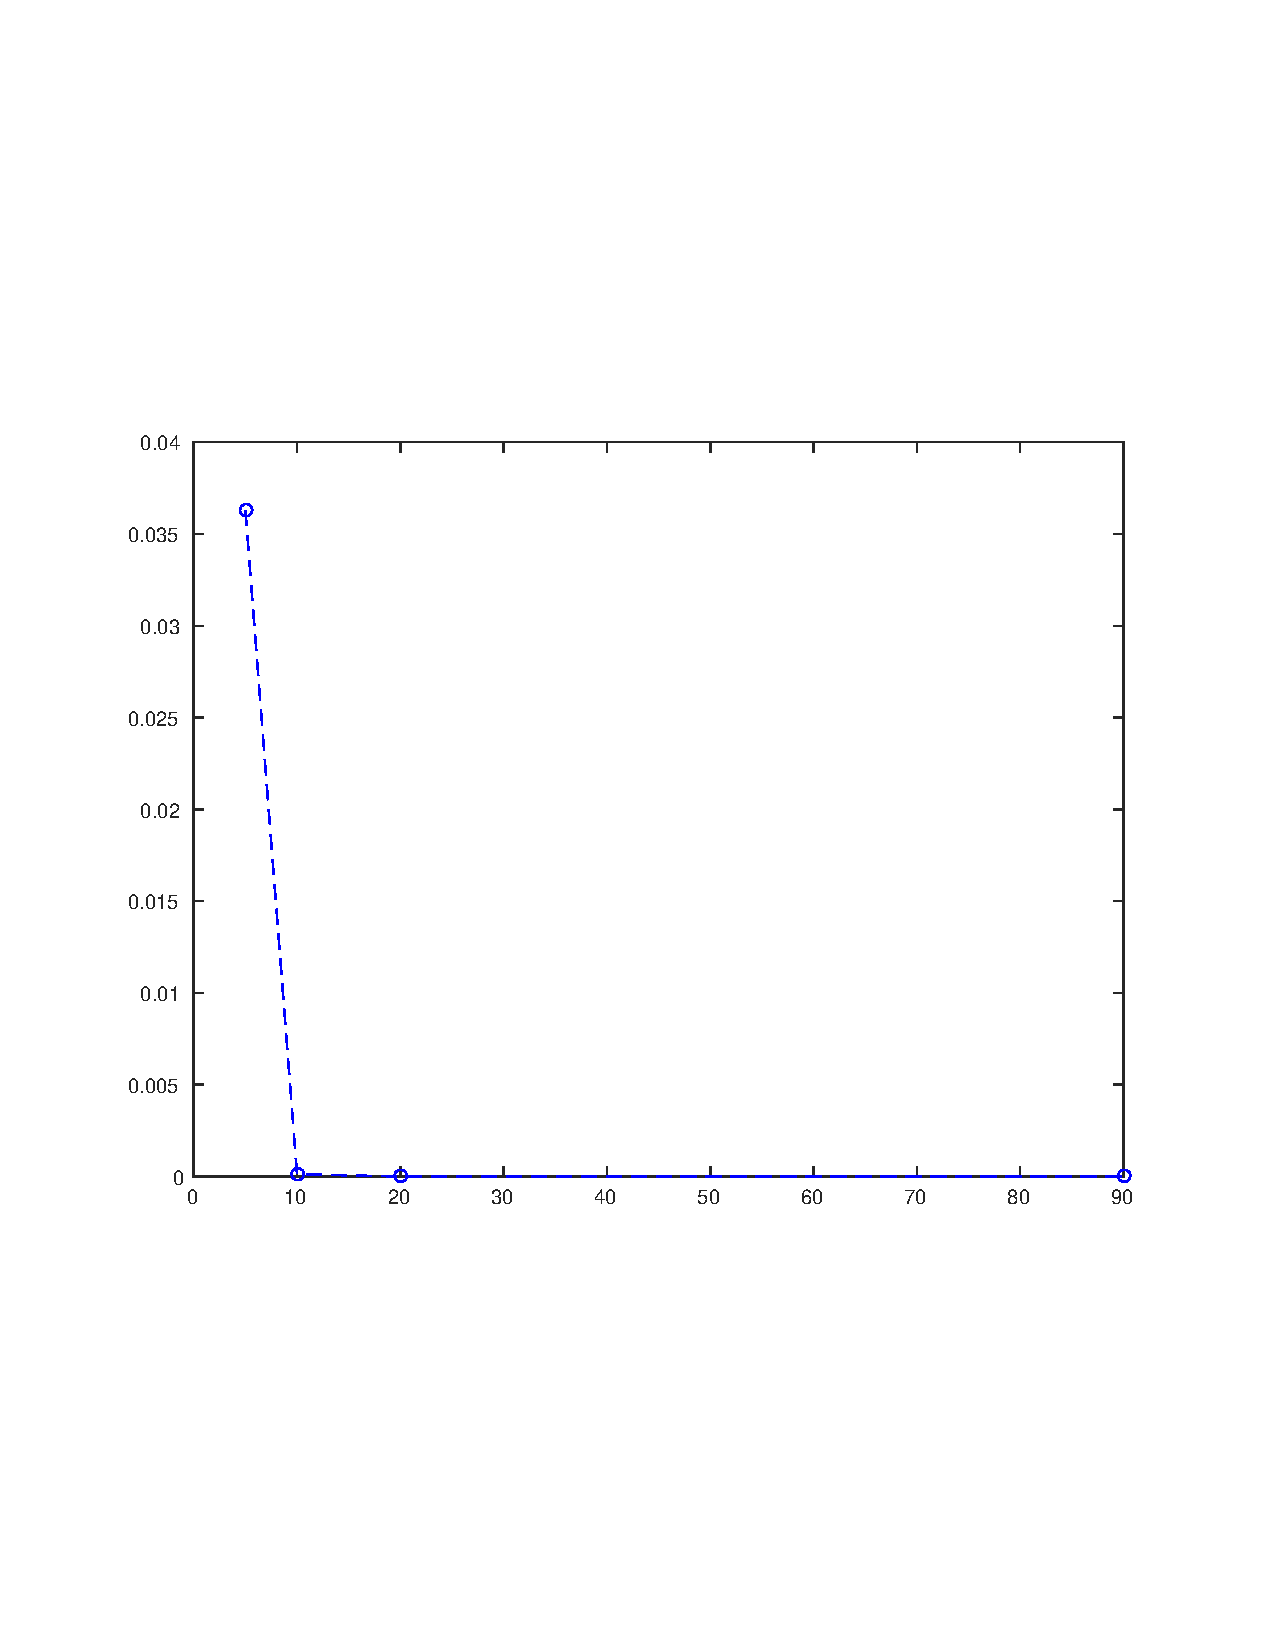
\includegraphics[trim=10mm 70mm 10mm 70mm, width=1.0\textwidth]{../q2_plots}
%\end{figure}
